\chapter{Large Scale Speech Recognition}
\label{chapter:largescale}

End to end speech recognition models are highly data hungry. \cite{Li2020OnRecognition}. Modern ASR systems have been designed to work in multiple domain and environment conditions, and this robustness is possible due to the usage of larger and larger datasets. One of the largest datasets that has been publicized is the 162,000 hours dataset from Google's research team. In their work, they have attempted to build a domain invariant speech recognition model using the large dataset\cite{Narayanan2019TowardTraining}. Other applications include multi-lingual ASR models \cite{Kannan2019Large-ScaleModel} and highly accurate domain specific ASR models. These experiments showcase the ability of the ASR systems to perform at high levels by using more and more data. An observation from almost all of these works is that the researches are limited to an industrial domain and published by Google, Microsoft, etc which have fewer budget constraint than other researchers in the domain of ASR. In the academic domain, the amount of research done in this direction is limited due to the resource constrains concerning disk storage, GPU resource, CPU resources, network communication and availability of datasets. 

\section{Scaling up training}
The major factor in the magnitude at which DNNs have grown is due to the increase in scaling of training them. There are three main dimensions in which this can be done. First is the magnitude of training data. The model performance can be improved by feeding more data to the deep neural network during training \cite{HestnessDEEPEMPIRICALLY}. The definition of a "large scale" dataset specific to speech recognition is ever-changing. For some context, a popular research in 2014 \cite{Hannun2014DeepRecognition}, used 5000 hours of training data and more recent research in 2020 \cite{Li2020OnRecognition}, researchers have used 160,000 hours of training data with random augmentation techniques for each epoch. In the previous 7 years, the training data used has grown by 32x. Increasing the amount of high-quality training data hence is one of the straightforward ways to improve performance of deep learning models. Hence, the practice of adding more and more training data is projected to continue through the next few years \cite{Mayer2020ScalableInfrastructures}. 

The second dimension is the scale of the infrastructure. The easily available parallel hardware, especially graphics processing units (GPUs), has proven to be a great enabler to train DNNs in shorter times than before \cite{ZhangPoseidon:Clusters}. This is due to the reducing costs of hardware resources and due to the boost in cloud computing. Storing and handling data have become cheaper and easier. GPU resources have become cheaper, which have enabled researchers to use more data for training of deep neural networks. 

The third dimension is the size of the DNN models, by increasing the width and depth of the models, DNN models have increased in complexity to achieve tremendous accuracies \cite{DeanLargeNetworks}. 

\section{Distributed Training}
To be competitive, it is clear that models have to be more complex and has to be trained on large datasets. Such huge training tasks can take models a few weeks or even months on a single GPU to reach convergence. To increase the throughput of the training system, one of the straightforward  methods is by increasing the amount of resources, which include the number of GPUs available. Distributed training is the method of training in a distributed infrastructure of multiple compute nodes, each with multiple GPUs on it\cite{Langer2020DistributedPerspective}. 

This also brings with it a number of challenges. The first challenge is to use the computing resources efficiently. This should also go along with tight integration of hardware elements to improve the throughput of the system. Data transmissions across machines are slow when performing transactions that are vital to train a network. During training a deep neural network using SGD, the weights have to be synchronized across all the devices in use. As the amount if GPUs in the system grows, the overhead also grows with it. These challenges require research at a confluence of both computing systems and deep learning training methods is receiving growing attention \cite{Xiao2018Gandiva:Learning, Mai2020KungFu:Adaptive, Chilimbi2014ProjectSystem, CuiGeePS:Server, Peng2018Optimus:Clusters}.

\subsection{Types of parallelism}
There are many ways to train deep learning models in parallel. The most common ones are discusses here, namely data and model parallelism.

\subsubsection{Model Parallelism}
In model parallelism, split the deep neural network into different devices and load a portion of the model on each device for training, as shown in Figure \ref{fig:modelparallel}. The device that holds the first layer receives the training data. Next, the data propagates through the rest of the forward pass on the device and the output of that device is passed to the next device that holds the next layer of the DL model. During the backward pass, compute the gradients starting from the device that hold the output layer and then propagate the gradients to the devices backward till the device with the input layer. 

\begin{figure}[ht]
  \begin{center}
    % below the size of the figure has been reduced for example
    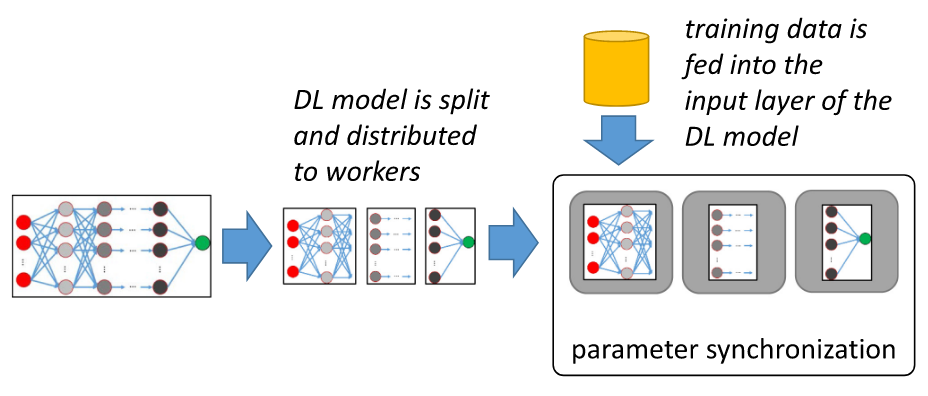
\includegraphics[width=\textwidth]{images/model parallelism.png} 
    \caption{Architecture Diagram of Model Parallelism  \cite{Mayer2020ScalableInfrastructures}}
    \label{fig:modelparallel}
  \end{center}
\end{figure}

The biggest challenge in model parallelism is to split the model into partitions that can be processed on different devices \cite{Mayer2017ThePath}. In many cases, the best way is to try out various permutations and measure the performance and keep the best permutation that has worked well. The second drawback is that model parallelism need heavy communication between devices. A combined effect of these two challenges is that stalling may occur if models are hard to be split effectively, to reduce the communication overloads and synchronization delays. Therefore, training speed might not increase linearly by increasing the number of parallel devices \cite{Mirhoseini2017DeviceLearning}.

The major benefit of the model parallelism is that it can accommodate huge deep learning networks, which cannot be stored on a single device (GPU) to train them because the memory required to train them is split to multiple devices. 

\subsubsection{Data Parallelism}
In data parallelism, copy the deep neural network into different devices and load an identical copy of the model on each device for training, as shown in Figure \ref{fig:dataparallel}. Split the data into the same number as the number of devices, and then data is passed into the model replicas of the workers for training. Perform the training process on each chunk of the data that is assigned to the device, which leads to updates of the model parameters. Once it is completed on the devices, the parameters need to be synchronized across all the devices. 

\begin{figure}[ht]
  \begin{center}
    % below the size of the figure has been reduced for example
    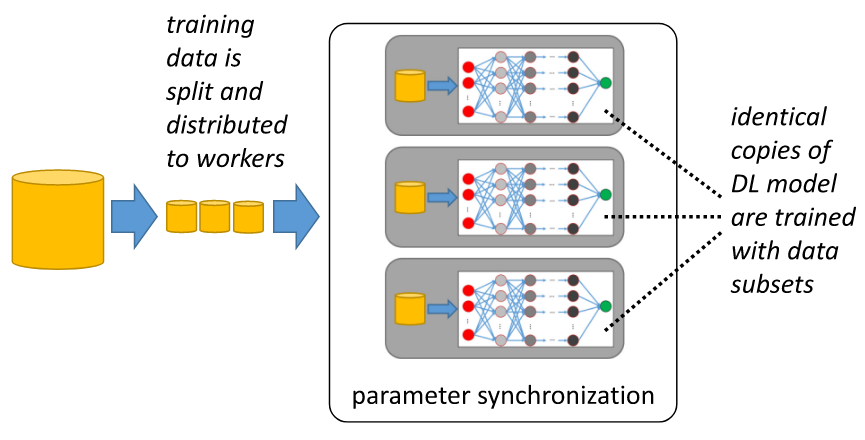
\includegraphics[width=\textwidth]{images/data parallelism.png} 
    \caption{Architecture Diagram of Data Parallelism  \cite{Mayer2020ScalableInfrastructures}}
    \label{fig:dataparallel}
  \end{center}
\end{figure}

Since on each device processes a mini batch of data, the total batch size is the product of the mini batch with the number of GPUs. This high data scale leads to poor convergence. The other drawback is that ideally the data that is split along the different workers needs to be identically distributed, so that the parameter updates by the different workers can be easily synchronized to get the overall model \cite{Jia2018BeyondNetworks}.

The major benefit of data parallelism is that it can be easily applied to most of the deep learning networks without much specific knowledge about the architecture of the model. It is highly scalable for the cases when the training is compute intensive but have relatively few parameters like RNNs, CNNs \cite{Krizhevsky2014OneNetworks}.

\subsection{Related Large scale ASR}

\section{Business Speech Dataset}

\subsection{Sharding}
\subsection{Sequential access}
\subsection{TAR advantages}
